\newpage
\section{Local Search}

% Introduzione
\subsection{Introduzione}

L'algoritmo di local search è di \hl{tipo euristico migliorativo}, cioè \textbf{presuppone che sia stata già prodotta una soluzione ammissibile}. 

Le \hl{procedure} da utilizzare si dividono in:

\begin{enumerate}
    \item \hl{single population}: \textbf{migliorare in un intorno (localmente) la situazione}, tenendo in conto che potrebbe rimanere bloccata in minimi locali
    \item \hl{multiple population}: ad ogni iterazione si ha un \textbf{insieme di soluzioni}
\end{enumerate}

Non essendo algoritmi precisi \hl{vanno adattati} al particolare problema che si intende affrontare.


% Progetto di ricerca locale
\subsection{Progetto di ricerca locale}

Si parte da una \hl{soluzione $x^{(0)}$} e si considera il suo \hl{intorno $N(x^{(0)}$}, cioè un \hl{insieme di soluzioni vicine a $x^{(0)}$} dove la definizione di "vicine" viene data dal progettista, aggiungiamo allora il vincolo:
$$\underline{x} \in N(\underline{x}^{(0)})$$


\begin{figure}[H]
\centering
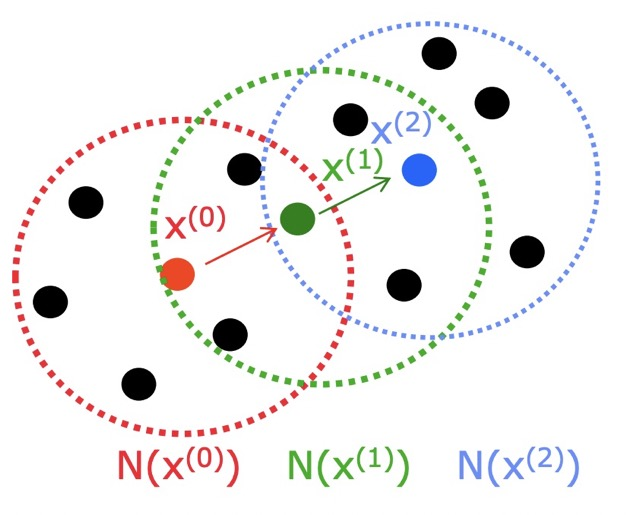
\includegraphics[scale=0.3]{localse.jpeg}
\caption{Local search} 
\label{localse}
\end{figure}


Avremo allora un problema con f.o:
$$\min z = \underline{c}^T\underline{x}$$
s.t.

\begin{itemize}
    \item $\underline{\underline{A}}\ \underline{x} \leq \underline{b}$
    \item $\underline{x} \geq 0$
    \item $\underline{x}$ integer
    \item $\underline{x} \in N(\underline{x}^{(0)})$
\end{itemize}

trovando così una soluzione $\underline{x}^{(1)}$ nell'intorno di $\underline{x}^{(0)}$, ecc ecc...

Sarà un algoritmo di \hl{discesa se minimizziamo} e di \hl{ascesa se massimizziamo}, ma entrambi si \hl{fermeranno in un ottimo locale}.


\begin{figure}[H]
\centering
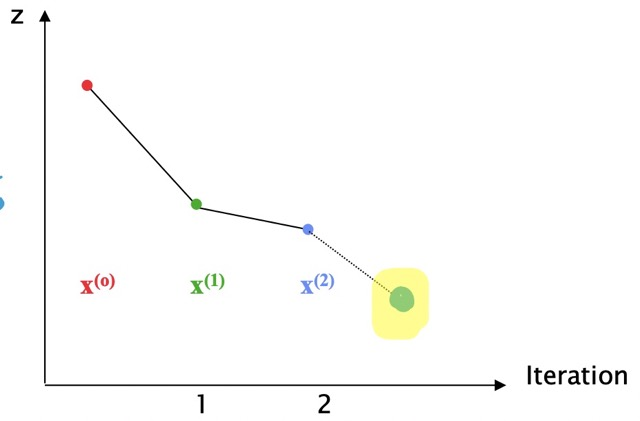
\includegraphics[scale=0.3]{stopsol.jpeg}
\caption{Esempio di ottimo locale} 
\label{stopsol}
\end{figure}


In questo caso un problema:

\begin{itemize}
    \item concavo: avrà un ottimo locale di \textbf{scarsa qualità}
    \item convesso: avrà un ottimo \textbf{uguale a quello globale}
\end{itemize}

Lo \hl{pseudocodice} nel caso di minimizzazione è:

\begin{itemize}
    \item[] INPUT: $\underline{x}^{(0)}$
    \item[] OUTPUT: $\underline{x}^{(k)}$
    \item[] $k = 0$
    \item[] repeat:
    \begin{itemize}
        \item[] solve $(P) + \text{constraint}\ \ \ \forall\ \ \ \underline{x}\in N(\underline{x}^{(k)})$
        \item[] let $\underline{x}^{(k+1)}$ be the optimal solution
        \item[] $k=k+1$
    \end{itemize}
    \item[] until: $z(x^{(k)})<z(x^{(k-1)})$
\end{itemize}

Riprendendo il problema del TSP dovremo \hl{definire un introno} sui punti:


\begin{figure}[H]
\centering
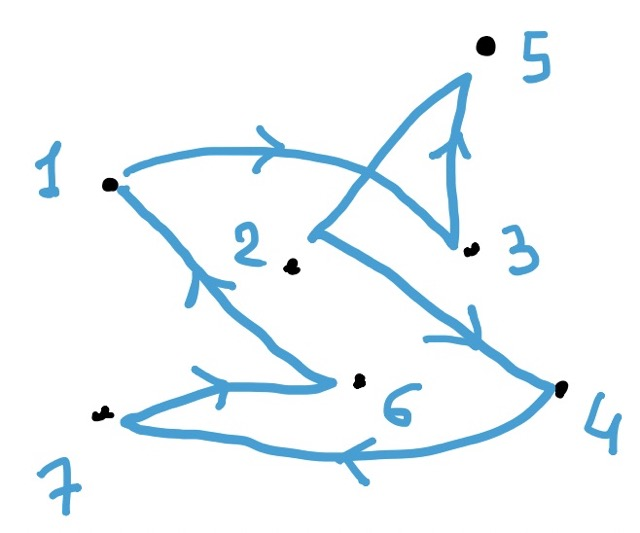
\includegraphics[scale=0.2]{intorno.jpeg}
\caption{Problema del TSP} 
\label{intorno}
\end{figure}


Dobbiamo \hl{definire una perturbazione della soluzione} quindi usiamo un approccio \hl{destroy and repair}:

\begin{enumerate}
    \item \hl{destroy}: \textbf{cancellare 2 archi} come $x_{13}$, $x_{25}$, creando una \hl{soluzione disconnessa} con punti $(1, 6, 7, 4, 2)$ e una con $(3, 5)$
    \item \hl{repair}: \textbf{creo una giunzione più efficiente} tra i due segmenti con $x_{15}$, $x_{23}$
\end{enumerate}

Questo potrebbe portare ad una \hl{variazione di costo}:
$$\text{var. costo } = \text{ archi aggiunti } - \text{archi tolti}$$
$$\Delta z = c_{15} + c_{23} - c_{13} - c_{25}$$


\begin{figure}[H]
\centering
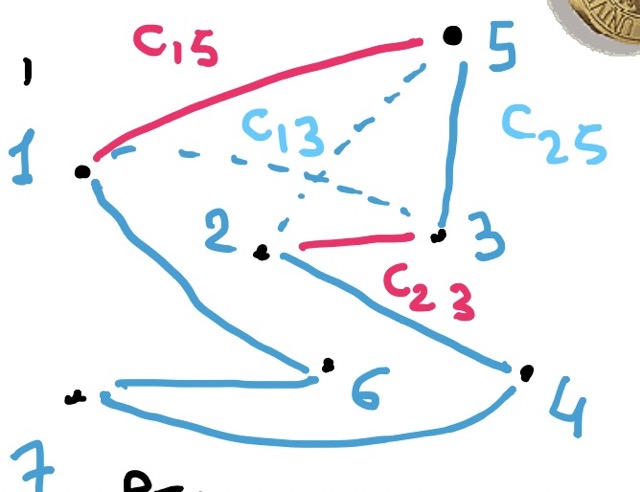
\includegraphics[scale=0.2]{intott.jpeg}
\caption{Ottimizzazione del problema TSP} 
\label{intott}
\end{figure}


L'intorno sarabbe l'\hl{insieme delle soluzioni ottenute dopo il dele and repair}. Quanto troviamo $\Delta z = 0$ ci fermiamo.


% Local branching
\subsection{Local branching}

Se troviamo un \hl{problema a grandi dimensioni} con \hl{variabili binarie}:
$$x1, ..., \in <0, 1>$$

Essendo un problema che \hl{richiederebbe una quantita' elevata di tempo}definiamo un \hl{intorno di un soluzione}. Volendolo dare in pasto ad un solver dobbiamo prima tradurre il vincolo $N(\underline{x}^{(k)})$  in forma di disequazione lineare, \hl{usando la distanza di Hamming} (conto i bit diveri tra due stringhe):

$$\underline{x}^{(k)} = (0,1,1,0,1,1)$$
$$\underline{x} = (1,1,1,0,0,1)$$

con distanza di Hamming: $d(\underline{x}, x^{(j)}) = 2 \text{bits}$.

Allora \hl{data una soluzione $\underline{x}^{(k)}$} avremo che:
$$\underline{x}\in N(\underline{x}^{(k)})\Leftrightarrow d(\underline{x}, \underline{x}^{(k)})\leq m$$

allora dovremo \hl{delle soluzioni $\leq m$}. La \hl{distanza di Hamming tra $\underline{x}$ e $\underline{x}^{(k)}$} sarà:
$$\sum_{j=1,...,n:x_j^{(k)}=0} x_j + \sum_{j=1,...,n:x_j^{(k)}=1} 1-x_j \leq m$$

o ancora meglio con: $\underline{x}k = (0, 1, 1, 0, 1, 1)$ \hl{possiamo contarli con}:
$$x_1 + (1-x_2) + (1-x_3) + x_4 + (1-x_5) + (1-x_6) \leq m$$
